\section{Hårdvara}\label{sec:hårdvara}
	Systemet är uppbyggt utav huvudsakligen tre komponenter: ett Digilent Nexys3 utvecklingskort, en
	temperperatursensor från Maxim och en mobiltelefon med serieinterface (\emph{RS232}).

	\subsection{Digilent Nexys3 - FPGA}
		Nexys3 är ett utvecklingkort från Digilent som bygger på en Spartan-6 FPGA från Xilinx.
		\\
		\textbf{Nexys3 har bland annat:}
		\begin{itemize}
			\item Xilinx Spartan-6 XC6SLX16 CSG324C.
			\item Klockfrekvens på 100MHz.
			\item 48MB externt minne, varav 32MB är ickeflyktigt.
			\item Mikro USB-port för programmering av FPGA och strömförsörjning.
			\item USB-UART, genom en mikro USB-port kopplad vid en FTDI FT232 krets.
			\item USB Host-kontroller för anslutning utav externa USB-enheter, ex. mus, tangentbort, osv.
			\item 10-100 Mbit ethernet-anslutning.
			\item 4st 7-segmentdisplayer.
			\item 8st binära DIP switchar.
			\item 8st ytmonterade lysdioder
			\item 4st kontaktstycken för externa I/O-enheter (dubbelbreda Pmod anslutningar).
		\end{itemize}
		
\begin{figure}[htp]
	\centering
	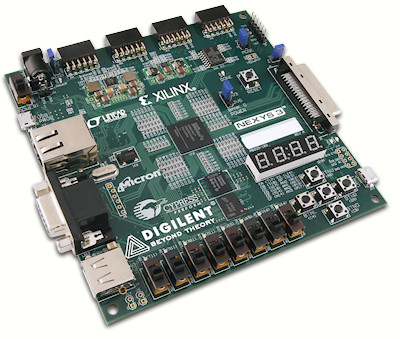
\includegraphics[scale=0.8]{nexys3.jpg}
	\caption{Digilent Nexys 3}
\end{figure}
		
		
		
		

\subsection{DS18S20 - Temperatursensor}\label{sec:hw:ds18s20}
DS18S20 är en temperatursensor tillvärkad av Dallas Semiconductor (numera Maxim) som enbart använder sig utav 1 pin för kommunikation. 
\\
\textbf{Sensorn har:}
\begin{itemize}
	\item Temperaturmätning från -75\degcel{} till 125\degcel{} med $\pm5$ precision.
	\item Alarmfunktion med icka-flyktigt minne.
	\item Max 750ms för temperaturmätning
	\item Flera sensorer kan dela på en buss.
	\item Ett unikt för varje enhet 64 bitars serienummer.
	\item Endast två pinnar behövs om ``parasite power'' anvands. Då laddar sensorn upp en kondensator när DQ drivs aktivt hög.
\end{itemize}
\begin{figure}[htp]
	\centering
	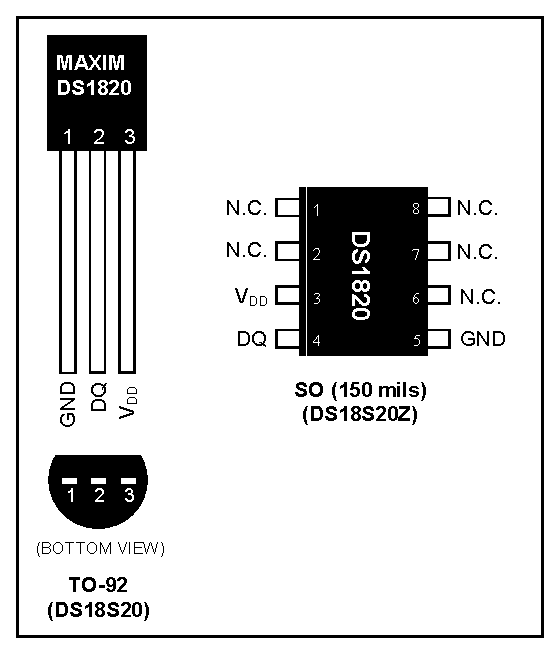
\includegraphics[scale=0.8]{ds18s20_hardware.eps}
	\caption{Dallas DS18S20}
\end{figure}
